\section{04.12.23 : Kategoria pochodna jako kategoria zlokalizowana}

\subsection{Quasi-izomorfizmy tworzą klasę lokalizującą}

\begin{theorem}
  qis tworzą w $K(\mathbf{A})$ klasę lokalizującą.
\end{theorem}

\begin{proof}
  \begin{enumerate}
    \item Składanie morfizmów jest oczywiste
    \item Uzupełniają się diagramy
      \begin{center}\begin{tikzcd}
        D^*\arrow[r, "qis" above]\arrow[d] & C^*\arrow[d, "g"] \\ 
        A^*\arrow[r, "s" above, "qis" below] & B^*
      \end{tikzcd}\end{center}

      \begin{center}\begin{tikzcd}
        {\color{red}(C(\tau))[-1]}\arrow[d, dashed]\arrow[r, dashed] & B^*\arrow[r, "\tau"], \arrow[d, phantom, sloped, "="] & C(s)\arrow[r]\arrow[d, phantom, sloped, "="] & C(\tau)\arrow[d] \\ 
        A^*\arrow[r, "s"] & B^*\arrow[r, "\tau"] &C(s) \arrow[r] & A^*[1]
      \end{tikzcd}\end{center}
      jest z poprzedniego wykładu, teraz chcemy do niego dopisać linijkę na górze

      \begin{center}\begin{tikzcd}
        C(\tau g)[-1]\arrow[r, green]\arrow[d] & C^*\arrow[d, "g"] \arrow[r, "\tau g"] & C(s) \arrow[d, phantom, sloped, "="] \arrow[r] & C(\tau g)\arrow[d, green] \\
        {\color{red}(C(\tau))[-1]}\arrow[d, dashed]\arrow[r, dashed] & B^*\arrow[r, "\tau"], \arrow[d, phantom, sloped, "="] & C(s)\arrow[r]\arrow[d, phantom, sloped, "="] & C(\tau)\arrow[d] \\ 
        A^*\arrow[r, "s"] & B^*\arrow[r, "\tau"] &C(s) \arrow[r] & A^*[1]
      \end{tikzcd}\end{center}

        Pojawia nam się szukany fragment (dwie pierwsze kolumny). Ponieważ $s$ jest qis, to $H^*(A^*)\to H^*(B^*)$ są izomorfizmami, a więc z ciągu dokładnego kohomologii wiemy, że $H^*(C(s))=0$. Ponieważ $C(s)$ jest takie samo na dole jak na górze, to wiemy, że $H^*(C(\tau g))[-1]\to H^*(C^*)$ jest izomorfizmem, co z definicji daje, że $C(\tau g)[-1]\to C^*$ jest qis.

      \item $sf=0$ w $K(\mathbf{A})$ (czyli $sf\overset{h}{\sim} 0$ w $Kom(\mathbf{A})$), to istnieje $t$ qis taki, że $ft=0$ w $K(\mathbf{A})$.

        Znowu rysujemy diagram 
        \begin{center}\begin{tikzcd} 
          &C(s)[-1]\arrow[d, phantom, sloped, "="] \arrow[r] & B^*\arrow[r, "s"] & \overline{B^*} \arrow[r] & C(s)\\ 
          C(g)&C(s)[-1]\arrow[l]& A^*\arrow[u, "f"]\arrow[l, "g"] & C(g)[-1]\arrow[l, "t"] \\ 
          &(f(a^i), -h(a^i))\arrow[u, sloped, phantom, "\in"] & a^i\arrow[l, mapsto]\arrow[phantom, sloped, u, "\in"]
        \end{tikzcd}\end{center}

        Jako ćwiczenie pozostaje sprawdzenie, że $gd=dg$.

        Ponieważ $s$ jest qis, to $C(s), C(s)[-1]$ są kompleksami acyklicznymi. Z tego wynika, że $t$ jest qis. 

        {\large\color{red}TUTAJ JESZCZE OBRAZKI ZE ZDJECIA}
  \end{enumerate}
\end{proof}

\subsection{Homotopie są tym samym w kat. pochodnej}

\begin{lemma}
  Niech $f,g:A^*\to B^*$ będą odwzorowaniami łańcuchowymi i $f\sim g$. Wtedy $Q(f)=Q(g)$, czyli indukują to samo w kategorii pochodnej $D(\mathbf{A})$.
\end{lemma}

Szybkie wytłumaczenie:
\begin{center}\begin{tikzcd}
   & f\sim g\\
  & Kom(\mathbf{A}) \arrow[dr, "Q"]\arrow[dl] \\ 
  K(\mathbf{A})[qis^{-1}] & & D(\mathbf{A})\arrow[ll]\\ 
  K(f)=K(g) & & Q(f), Q(g)\arrow[ll, mapsto]
\end{tikzcd}\end{center}

\begin{definition}
  Jeśli $A^*$ jest kompleksem, to kompleks $A^*\times I$ jest definiowany jako 
  $$(A^i\times I)^i=A^i\oplus A^{i+1}\oplus A^i$$
  z różniczką
  $$d(a^i, a^{i+1}, a'^i)=(da^i-a^{i+1}, -da^{i+1}, da'^i+a^{i+1})$$
\end{definition}

Tak zdefiniowany kompleks $A^*\times I$ jest związany z kompleksem $A^*$, m.in. istnieją włożenia i rzuty:
\begin{center}\begin{tikzcd}
  & (a^i, 0, 0) \\
  a^i\arrow[ur, "i_0"] \arrow[dr, "i_1"]& & & (a^i, a^{i+1}, a'^i)\arrow[r, mapsto, "p"] & (a^i+a'^i)\\ 
  & (0, 0, a^i)
\end{tikzcd}\end{center}

\begin{lemma}[a dokładniej to podlemat]
  $i_0p\sim id_{A^*\times I}\sim i_1p$, zatem $i_0$ oraz $i_1$ są qis odwrotnymi do qis $p$. W takim razie w kategorii pochodnej $D(\mathbf{A})$ mamy 
  $$Q(p)^{-1}=Q(i_0)=Q(i_1)$$
\end{lemma}

\begin{proof}
  Dowód dla $i_0$:
  \begin{align*}
    h(a^i, a^{i+1}, a'^i)&=(0, a'^i, 0)\\ 
    dh(a^i, a^{i+1}, a'^i) &= (-a'^i, -da'^i, a'^i)\\ 
    hd(a^i, a^{i+1}, a'^i) &= (0, da'^i+ a^{i+1}, 0)\\ 
    dh+hd (a^i, a^{i+1}, a'^i)&=()
  \end{align*}


\begin{center}\begin{tikzcd}
  & (a^i+a'^i, 0, 0) \arrow[dr]\\
  (a^i, a^{i+1}, a'^i)\arrow[ur, "i_0p"] \arrow[dr, "id"] & & (-a'^i, a^{i+1}, a'^i) \\ 
  & (a^i, a^{i+1}, a'^i)\arrow[ur]
\end{tikzcd}\end{center}
Czyli $dh+hd=id-i_0p$.

\end{proof}

\begin{proof}
  Dowód lematu wyżej.

  Niech $f\overline{h}{\sim} g$. Przerobimy to na $H:A^*\times I\to B^*$ tak, że 
  $$Hi_0=f, Hi_1=g.$$
  Wzorem zapisuje się to 
  $$H(a^i, a^{i+1}, a'^i)=f(a^i)+h(a^{i+1})+g(a'^i).$$
  Chcemy sprawdzić, że jest to łańcuchowe. 
  \begin{center}\begin{tikzcd}
    (a^i, a^{i+1}, a'^i) \arrow[r, "H"]\arrow[d, "d"] & {\color{red}f(a^i)} +h(a^{i+1})+{\color{red}g(a'^i)}\\ 
    ({\color{green}da^i-a^{i+1}}, -da^{i+1}, da'^i+a^{i+1}) \arrow[r, "H"] & \substack{
      {\color{green}(}{\color{red}df(a^i)}-f(a^{i+1}){\color{green})}+ \\ -hda^{i+1}+ \\ +{\color{red}dg(a^i)}+g(a^{i+1})
    }
  \end{tikzcd}\end{center}
  $$Q(f)=Q(Hi_0)=Q(H)Q(i_0)=Q(H)Q(i_1)=Q(Hi_1)=Q(g)$$
\end{proof}

\subsection{Równoważność domków i qis}

\begin{fact}
  $$K(\mathbf{A})[qis^{-1}]=D(\mathbf{A})$$
\end{fact}

\begin{proof}
  Zaczynamy od diagramu, na którym się to wszystko opiera 
  \begin{center}\begin{tikzcd}
    & Kom(\mathbf{A}) \arrow[dl] \arrow[dr, "Q"] \\ 
    K(\mathbf{A})[qis^{-1}] & & D(\mathbf{A})\arrow[ll]
  \end{tikzcd}\end{center}
  na obiektach to wszystko jest identycznością. Na morfizmach strzałka $D(\mathbf{A})\to K(\mathbf{A})[qis^{-1}]$ jest surjektywna: $Q(f)Q(s)^{-1}$ przechodzi na element
  \begin{center}\begin{tikzcd}
    & B\arrow[dl, "s" above left]\arrow[dr, "f"] &    &   & B\arrow[dl, "s" above left] \arrow[dr, "id"] &   & B\arrow[dl, "id" above left]\arrow[dr, "f"] \\ 
    A &                               & A' & A &                                   & B & & A
  \end{tikzcd}\end{center} 
  Chcemy teraz pokazać, że $D(\mathbf{A})\to K(\mathbf{A}[qis^{-1}]$ jest też $1-1$. Z każdego morfizmu w $D(\mathbf{A})$ pojawi się domek w $K(\mathbf{A})[qis^{-1}]$. Każda strzałka w $D(\mathbf{A})$ to jeden domek. Ale ponieważ umiemy domki składać, to 
  \begin{center}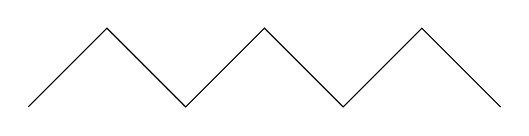
\begin{tikzpicture}
    \draw(0, 0)--(1, 1)--(2, 0)--(3, 1)--(4, 0)--(5, 1)--(6, 0);
  \end{tikzpicture}\end{center}
  {\large\color{red}TUTAJ OBRAZKI ZE ZDJĘĆ}

  Każdy morfizm w $D(\mathbf{A})$ jest dany domkiem postaci 
  \begin{center}\begin{tikzcd}
    & .\arrow[dl, "S"]\arrow[dr, "F"]\\ 
    . & & . 
  \end{tikzcd}\end{center}
  gdzie $S$ jest qis. To znaczy, że każdy domek jest postaci $Q(F)Q(S)^{-1}$. Załóżmy więc, że mamy diagram
  \begin{center}\begin{tikzcd}
    B\arrow[r, "F"]\arrow[d, "S"] & A'\\ 
    A & B'\arrow[l, "S'"] \arrow[u, "F'"]
  \end{tikzcd}\end{center}
  gdzie góra i dół przechodzi na to samo, mianowicie
  \begin{center}\begin{tikzcd}
      &   & C\arrow[dl, "T"] \arrow[dr, "G"] \\ 
      & B \arrow[dl, "S"]\arrow[drrr, "F"] & & B' \arrow[dr, "F'"]\arrow[dlll, "S'"] \\ 
    A &   & &   & A'
  \end{tikzcd}\end{center}
  \begin{align*}
    Q(F)Q(S)^{-1}&=Q(F)Q(T)Q(T)^{-1}Q(S)^{-1}=Q(FT)Q(ST)^{-1}=Q(F'G)Q(ST)^{-1}= \\ 
                 &=Q(F'G)Q(S'G)^{-1})=Q(F')Q(G)Q(G)^{-1}Q(S')^{-1}=Q(F')Q(S')^{-1}
  \end{align*}
\end{proof}

\begin{example}
\item $A=Vect_K$, wtedy 
  $$D(\mathbf{A})=\prod_{n=-\infty}^\infty \mathbf{A}[n]=Kom_0(\mathbf{A})$$
  to po prawej to kompleksy łańcuchowe z zerowymi różniczkami.

  \begin{center}\begin{tikzcd}
    Kom(\mathbf{A}) \arrow[rr, "H^*", yshift=1mm] \arrow[dr] & & Kom_0(\mathbf{A})\arrow[ll, yshift=-1mm, hookrightarrow]\arrow[dl, "l" above left, yshift=1mm] \\ 
       & D(\mathbf{A})\arrow[ur, "k" below right, yshift=-1mm]
  \end{tikzcd}\end{center}
  Tutaj $lk\sim id_{D(\mathbf{A})}$ jest homotopijne.
\end{example}

\subsection{Pomiędzy nami, obiektami, a wszystkimi kompleksami}

\begin{definition}
  $A^*\in Kom(\mathbf{A})$ jest $H^0$-kompleksem, jeśli $H^i(A^*)=0$ dla $i\neq 0$.
\end{definition}

\begin{fact}\label{fakt 10.5}
  Jeśli popatrzymy na funktor $\mathbf{A}\to D(\mathbf{A})$
  $$A\mapsto (...\to 0\to A\to 0\to ...)$$
  to taki funktor jest równoważnością między $A$ i pełną podkategorią $D(\mathbf{A})$ rozpiętą na $H^0$-kompleksach.
\end{fact}

$(...\to0\to A\to0\to...)$ oznacza się $A[0]$ lub nawet $A$.

\begin{proof}
  Nazwijmy badany funktor $F$. Pokażemy, że jest on wiermy, pełny i w zasadzie surjektywny.

  $$Hom_{\mathbf{A}}(X, Y)=Hom_{K(\mathbf{A})}(X, Y)$$
  są praktycznie takie same, bo jeśli $\phi: X\to Y$, to po prawej stronie mamy
  \begin{center}\begin{tikzcd}
    ...\arrow[r] & 0\arrow[r] \arrow[d] & X\arrow[r]\arrow[d, "\phi"] \arrow[dl, blue] & 0\arrow[r] \arrow[d] \arrow[dl, blue] & ... \\ 
    ...\arrow[r] & 0\arrow[r] & Y \arrow[r] & 0\arrow[r] & ...
  \end{tikzcd}\end{center}
  i wszystkie możliwe homotopie są między $0$ lub z/do $0$, więc one same też są zerowe.

  Dalej niech \begin{tikzcd}Hom_{K(\mathbf{A})}(X, Y)\arrow[r, yshift=1mm, "a"] & Hom_{D(\mathbf{A})}(X, Y)\arrow[l, "b=H^0", yshift=-1mm]\end{tikzcd}. Od razu można zauważyć, że $b\circ a=id$, więc pytamy tylko o $a\circ b$. Mamy 
  {\large\color{red}KOLEJNY RYSUNEK}
\end{proof}
